\chapter{Kripke结构、时序逻辑、模型检测以及遗忘理论}\label{chapter02}

{\em 本章主要介绍本文用到的符号、术语以及逻辑理论基础,包括:Kripke结构、时序逻辑(尤其是计算树逻辑(CTL)和$\mu$-演算)、模型检测和遗忘理论。首先,介绍解释时序逻辑语言所需的模型结构,即Kripke结构。其次,主要介绍时序逻辑中本文探讨的计算树逻辑和$\mu$-演算。为了更加明确本文的研究动机,本章将详细介绍模型检测的基本概念和一些主要的性质。此外,遗忘理论是本文的研究重点,其概念、性质及在各个研究领域的研究和应用情况将会被当作本章的重点详细介绍。

为了方便,本文将命题变量(也叫原子命题)的集合记作$\cal A$,$V\subseteq {\cal A}$ 是$\cal A$的子集。此为,规定$\overline{V}$是$V$在${\cal A}$上的补,也即是$\overline{V}={\cal A}-V$。}
%{\em 围绕差分隐私应用中存在的隐私与数据可用性之间的权衡问题,本文以隐私信息度量为基础,试图从均衡优化的角度提供一种解决方案。为了更好的阐述后续的研究内容,本章首先介绍本文工作所需的基本模型与定义,包括隐私定义、差分隐私模型的形式化定义、Shannon信息论的基本通信模型及信息熵的概念。随后,介绍信息论、优化理论与对策博弈的基础知识,并以此为基础介绍了差分隐私均衡优化主要研究问题的描述及定义。本章阐述的内容主要为后续章节的具体研究奠定基础。}

\section{Kripke结构}
Kripke结构作为一种表示转换系统(transition system)的数学模型,在理论计算机科学领域有着广泛的应用,尤其是作为解释时序逻辑公式的模型结构。

\subsection{真假赋值和K-解释}
经典命题语言${\cal L}^p$由以下三类符号构成:
\begin{itemize}
	\item 命题符号:一般用小写拉丁字母$p$,$q$,$r$,$\dots$来表示,且这些命题符号来源于$\Ha$;
	\item 联结符号:$\neg$(否定),$\wedge$(合取),$\vee$(吸取),$\rto$(蕴涵),$\lrto$(等值于);
	\item 标点符号:((左括号),)(右括号)。
\end{itemize}
%命题符号:一般用小写拉丁字母$p$,$q$,$r$,$\dots$来表示,且这些命题符号来源于$\Ha$;
%连接符号:$\neg$(否定),$\wedge$(合取),$\vee$(吸取),$\rto$(蕴涵),$\lrto$(等值于);
%标点符号:((左括号),)(右括号)。

${\cal L}^p$的原子公式的集合和公式的集合分别记作$Atom({\cal L}^p)$和${\cal F}({\cal L}^p)$。其中,$Atom({\cal L}^p)$是命题符号的集合,且$\varphi\in {\cal F}({\cal L}^p)$当且仅当它能由(有限次使用)以下的三条规则生成\cite{luzhongwan1989}:
\begin{itemize}
	\item 如果$\varphi\in Atom({\cal L}^p)$,则$\varphi \in {\cal F}({\cal L}^p)$。
	\item 如果$\varphi \in {\cal F}({\cal L}^p)$,则$(\neg \varphi)\in {\cal F}({\cal L}^p)$。
	\item 如果$\varphi$,$\varphi'\in {\cal F}({\cal L}^p)$,则$(\varphi * \varphi')\in {\cal F}({\cal L}^p)$。其中,$*\in \{\wedge,\vee, \rto, \lrto\}$。
\end{itemize}
此外,也称“ture”和“false”为原子公式,分别记为“$\top$”和“$\bot$”。原子命题或其否定称为\emph{文字},有限个文字的吸取称为\emph{子句}。

\begin{example}\label{exp:pro:form}
	下面几个字符串为${\cal L}^p$的公式:
	\begin{itemize}
		\item $(q \vee p)$;
		\item $(((\neg p)\lrto(q\vee r))\rto(r \wedge p))$。
	\end{itemize}
	而字符串$p\wedge \vee q$不属于集合$\varphi\in {\cal F}({\cal L}^p)$。
\end{example}


为了方便,称${\cal L}^p$的公式为\emph{命题公式}(在不引起歧义的情况下也称之为\emph{公式})。此外,规定联结符号的优先级有助于简化公式(省略掉冗余的标点符号)。为此,规定在下面的序列中,每个左边的联结符号优先于右边的联结符号。
\[
\neg \qquad \wedge \qquad \vee \qquad \rto \qquad \lrto
\]
此时,例~\ref{exp:pro:form}中的公式$(((\neg p)\lrto(q\vee r))\rto(r \wedge p))$就可写为$(\neg p \lrto q \vee r) \rto r \wedge p$。当然,为了看起来方便,有的括号可以不必省略。

在讨论了命题公式的语法结构之后,接下来将讨论其语义解释。

\begin{definition}[真假赋值]\label{def:pro:interp}
	真假赋值是以所有命题符号的集为定义域,以真假值的集$\{0,1\}$为值域的函数$v:{\cal A}\rto \{0,1\}$。
\end{definition}
为了方便,后文中也将$\top$代表$1$,$\bot$代表$0$(此时真假赋值为$v:\Ha \rto \{\bot, \top\}$),且满足对任意的真假赋值$v$都有$\top^v=1$和$\bot^v=0$。由该定义可知,真假赋值的个数为$2^{|{\cal A}|}$个,因为一个真假赋值要同时给${\cal A}$中的所有命题符号指派一个真假值。真假赋值$v$给公式$\varphi$指派的值记作$\varphi^v$,其被形式化定义为如下:
\begin{definition}[公式的真假值]\label{def:pro:vformula}
	真假赋值$v$给公式指派的真假值递归定义如下:
	\begin{itemize}
		\item $p^v\in \{\bot,\top\}$,其中$p\in\Ha$。
		\item $(\neg \varphi)^v=\left\{
		\begin{array}{ll}
			\top, \qquad \hbox{如果$\varphi^v=\top$;} \\
			\bot,  \qquad  \hbox{否则。}
		\end{array}
		\right.$
		\item $(\varphi \wedge \psi)^v=\left\{
		\begin{array}{ll}
			\top, \qquad \hbox{如果$\varphi^v=\psi^v=\top$;} \\
			\bot,  \qquad  \hbox{否则。}
		\end{array}
		\right.$
		\item $(\varphi \vee \psi)^v=\left\{
		\begin{array}{ll}
			\top, \qquad \hbox{如果$\varphi^v=\top$或$\psi^v=\top$;} \\
			\bot,  \qquad  \hbox{否则。}
		\end{array}
		\right.$
		\item $(\varphi \rto \psi)^v=\left\{
		\begin{array}{ll}
			\top, \qquad \hbox{如果$\varphi^v=\bot$或$\psi^v=\top$;} \\
			\bot,  \qquad  \hbox{否则。}
		\end{array}
		\right.$
		\item $(\varphi \lrto \psi)^v=\left\{
		\begin{array}{ll}
			\top, \qquad \hbox{如果$\varphi^v=\psi^v$;} \\
			\bot,  \qquad  \hbox{否则。}
		\end{array}
		\right.$
	\end{itemize}
\end{definition}
对于任意的命题公式$\varphi$和真假赋值$v$,当$\varphi^v=\top$时,称$v$是公式$\varphi$的一个模型,也可以记为$v \models \varphi$,读作$v$满足$\varphi$。一般地,当存在一个真假赋值$v$使得$v\models \varphi$,则称公式$\varphi$是\emph{可满足的}。如果$\varphi$是可满足的,且$\neg \varphi$是不可满足的,则称$\varphi$是\emph{有效的}。

值得注意的是,命题逻辑的语义也可定义在“解释(interpretation)”上。一个\emph{解释}$I$是$\Ha$的子集。除了对原子命题$p\in \Ha$,$I$对公式的解释如真假赋值一样。在解释原子命题$p\in \Ha$上,$p^I$为真当且仅当$p\in I$。模型和可满足的定义与真假赋值的类似。

模态逻辑是经典逻辑的扩充,它是经典逻辑中引进“必然”和“可能”这两种模态词得到的。如上所述,命题的真假值只有两种,命题是真的(1)或是假的(0)。而在模态逻辑中,把命题
区分为必然真的命题和并非必然真的命题,把假命题区分为必然假的和并非必然假的命题。对于任何命题$\varphi$,可以有两种模态命题:“$\varphi$是必然的”和“$\varphi$是可能的”。值得注意的是,时序逻辑也是模态逻辑的一种。

本文所说的模态逻辑为命题单模态逻辑(propositional mono-modal logic)。模态公式的集合${\cal F}^{\Hm}$是包含“$\top$”和“$\bot$”的满足如下条件的最小集:
\begin{itemize}
	\item $\Ha \subseteq {\cal F}^{\Hm}$;
	\item 如果$\varphi \in {\cal F}^{\Hm}$,则$(\neg \varphi)$,$(\MPK \varphi)\in {\cal F}^{\Hm}$;
	\item 如果$\varphi$,$\psi\in {\cal F}^{\Hm}$,则$(\varphi * \psi)\in {\cal F}^{\Hm}$,其中$*\in \{\wedge,\vee, \rto, \lrto\}$。
\end{itemize}
令$\MPB = \neg \MPK \neg$,则$\MPB \varphi \in {\cal F}^{\Hm}$。其中,$\MPK$和$\MPB$叫做模态符号,分别表示“必然”和“可能”。

\emph{可能世界语义}(或\emph{Kripke语义})是标准的命题模态逻辑语义\cite{kripke1963semantical}。Kripke语义是定义在Kripke结构上的,一个Kripke结构是一个三元组$(S,R,L)$(下一节中将详细介绍)。
其中,$S$是状态的非空集合,$R\subseteq R \times R$是可达性关系。特别地,当$R$是一个等价关系的时候(模态逻辑S5中),一个Kripke结构可以写成一个二元组$\tuple{W,w}$,其中$W$是状态的非空集合,$w$是$W$中的元素,每个状态是原子命题的集合。此时,称$\Hm=\tuple{W,w}$为一个$\MPK$-\emph{解释}($\MPK$-interpretation)\cite{zhang2009knowledge}。

%$\MPK-$解释和${\cal F}^{\Hm}$种公式的可满足关系被归纳定义如下:
\begin{definition}\label{def:s5:interp}
	给定一个$\MPK$-解释$\Hm=\tuple{W,w}$,其与${\cal F}^{\Hm}$中的公式的可满足关系被归纳地定义为:
	\begin{itemize}
		\item $\Hm \not \models \bot$,$\Hm \models \top$;
		\item $\Hm \models p$当且仅当$p\in w$,其中$p\in \Ha$;
		\item $\Hm \models \neg \varphi$当且仅当$\Hm \not \models \varphi$;
		\item $\Hm \models \varphi \supset \psi$当且仅当$\Hm \not \models \varphi$或$\Hm \models \psi$;
		\item $\Hm \models \MPK \varphi$当且仅当$\forall w'\in W$有$\tuple{W, w'}\models \varphi$。
	\end{itemize}
\end{definition}

$\Hm=\tuple{W,w}$称为公式$\varphi$的$\MPK$-\emph{模型}($\MPK$-model),当且仅当$\Hm \models \varphi$。此外,如果存在一个$\Hm=\tuple{W,w}$使得公式$\Hm\models \varphi$,则称公式$\varphi$是可满足的。如果$\Hm\models \varphi$对于所有的$\Hm=\tuple{W,w}$都成立,则称$\varphi$是有效的。


\subsection{Kripke结构的定义及相关术语}
通常一个转换系统(transition system)能够被抽象为一个Kripke结构\cite{Baier:PMC:2008}。如上文所说,一个Kripke结构是一个三元组$\Hm=(S,R,L)$,其中:
\begin{itemize}
	\item $S$是状态的非空集合;
	\item $R \subseteq S \times S$是状态转换函数;
	\item $L:S\rto 2^{\Ha}$是一个标签函数。
\end{itemize}
在本文中,要求$R$是一个串行关系(serial relation),也即是对于$S$中的任意元素$s$,都存在$S$中的一个元素$s'$使得$(s,s')\in R$。

给定一个Kripke结构$\Hm=(S,R,L)$,$\Hm$上的一条\emph{路径}是一个无限的状态序列$\pi=(s_0,s_1,\dots)$且满足对于任意的$j\ge 0$都有$(s_j,s_{j+1})\in R$,路径上的状态$s$被记为$s\in \pi$。当给路径$\pi$引入一个状态$s$作为下标,记为$\pi_s$,则称该路径是起点为该状态$s$的一条路径。如果对于$\Hm$中的任意状态$s'$,都有一条以$s$为起点的路径$\pi_{s}$使得$s'\in \pi_{s}$,那么称状态$s$为一个\emph{初始状态}。给定$s_0$为$\Hm$中的一个初始状态,为了容易看出该初始状态,将该Kripke结构写为四元组$(S,R,L,s_0)$,并称该结构为\emph{初始结构}以区分于原来的三元组。

\emph{树}是一种只有一个根节点(没有其他节点指向且可达于其他节点的节点)无环图。
给定一个初始结构$\Hm=(S,R,L,s_0)$和一个状态$s\in S$,定义在$\Hm$上以$s$为根节点的深度为为$n$($n\ge 0$)的\emph{计算树}$\Tr_n^{\Hm}(s)$被递归定义如下\cite{browne1988characterizing}:
\begin{itemize}
	\item $\Tr_0^{\Hm}(s)$ 是只有一个节点$s$(其标签为$L(s)$)树。
	\item $\Tr_{n+1}^{\Hm}(s)$是以$s$为根节点(标签为$L(s)$)的树,并且满足若$(s,s')\in R$,则节点$s$有一棵子树$\Tr_{n}^{\Hm}(s')$。
\end{itemize}
%深度为$n$的\emph{计算树}$\Tr_n^{\Hm}(s)$是定义在初始结构$\Hm=(S,R,L,s_0)$和状态$s\in S$上的一个分支结构

一个初始结构$\Hm=(S,R,L,s_0)$和一个状态$s\in S$构成一个$\MPK$-\emph{结构}(或$\MPK$-解释),写作${\cal K}=(\Hm,s)$。
在$\MPK$-结构${\cal K}=(\Hm,s)$中,若$s=s_0$,则称该$\MPK$-结构为\emph{初始$\MPK$-结构},此时有${\cal K}=(\Hm,s_0)$。



\section{时序逻辑}
时序逻辑是一种描述系统规范的形式化语言,它研究状态随时间变化的系统的逻辑特性。由于软件和硬件的运行的本质是状态变化的过程,所以时态逻辑在软件程序验证和硬件验证中应用得相当广泛。计算树逻辑(Computation Tree Logic, $\CTL$)是分支时态逻辑的一种,其模型检测是多项式时间可行的。然而,$\CTL$表达系统性质的表达能力不如$\mu$-演算($\mu$-calculus),如:“某给定的系统中存在一条路径使得该路径上的第偶数个状态满足特定的性质”这一规范是不能用其他时态逻辑表示的[18]。充分考虑这两种逻辑语言自身的特性,本节主要介绍$\CTL$和$\mu$-演算。因此,本文所说的公式指$\CTL$(或$\mu$-演算)公式,即用来描述一个规范(或性质)的公式是$\CTL$(或$\mu$-演算)公式。

\subsection{计算树逻辑(\CTL)}
$\CTL$由Clark和Emerson等人于1986年提出\cite{DBLP:journals/toplas/ClarkeES86}。$\CTL$的语言${\cal L}$由下面的几类符号构成:
\begin{itemize}
	\item 原子命题的集合$\Ha$;
	\item 常量符号:$\top$和$\bot$;
	\item 经典联结符号:$\vee$和$\neg$;
	\item 路径量词:$\ALL$和$\EXIST$;
	\item 时序操作符:$\NEXT$、$\FUTURE$、$\GLOBAL$、$\UNTILL$和$\UNLESS$,分别表示“下一个状态”、“将来某一个状态”、“将来所有状态”、“直到”和“除非”;
	\item 标点符号:“(”和“)”。
\end{itemize}
$\CTL$的时序算子是路径量词和时序操作符的组合(路径量词在前,时序操作符在后),如:$\ALL \NEXT$,$\EXIST \NEXT$, $\ALL \FUTURE$等。
与经典命题逻辑一样,给联结符号规定优先级,有时候会带来意想不到的方便。$\CTL$中的联结符号的优先级如下序列所示,每个左边的联结符号优先于右边的联结符号:
\[
\neg \quad \EXIST\FUTURE \quad \EXIST\GLOBAL \quad \ALL\NEXT \quad \ALL\FUTURE \quad \ALL\GLOBAL \quad \wedge \quad \vee \quad \EXIST\UNTILL \quad \EXIST\UNLESS \quad \ALL\UNLESS \quad \rto
\]

因此,语言$\cal L$的\emph{存在范式(existential normal form, ENF)}可以用巴科斯范式递归定义如下:
\begin{equation}\label{def:CTL:formulas}
	\phi ::=  \bot \mid \top \mid p \mid\neg\phi \mid \phi\lor\phi \mid
	\EXIST \NEXT \phi \mid
	\EXIST \GLOBAL \phi \mid
	\EXIST (\phi\ \UNTILL\ \phi)
\end{equation}
其中,$p\in \Ha$。$\cal L$中其他形式的公式可以通过下面的定义(使用上述定义中(\ref{def:CTL:formulas})的形式)得到:
\begin{alignat}{2}
	 \varphi \wedge \psi& \ \overset{def}{=}\ \neg (\neg \varphi \vee \neg \psi)\\
	 \varphi \rto \psi& \ \overset{def}{=}\ \neg \varphi \vee \psi\\
	 \ALL(\varphi \UNTILL \psi)& \ \overset{def}{=}\ \neg\EXIST(\neg \psi \UNTILL(\neg \varphi \wedge \neg \psi)) \wedge \neg \EXIST \GLOBAL \neg \psi\\
	 \ALL(\varphi \UNLESS \psi)& \ \overset{def}{=}\  \neg\EXIST((\varphi \wedge \psi) \UNTILL (\neg \varphi \wedge \neg \psi))\\
	 \EXIST(\varphi \UNLESS \psi)& \ \overset{def}{=}\  \neg\ALL((\varphi \wedge \psi) \UNTILL (\neg \varphi \wedge \neg \psi))\\
	 \ALL\FUTURE \varphi& \ \overset{def}{=}\ 	\ALL(\top \UNTILL \psi)\\
	 \EXIST\FUTURE \varphi& \ \overset{def}{=}\ \EXIST(\top \UNTILL \psi)\\
	 \ALL \NEXT \varphi& \ \overset{def}{=}\  \neg \EXIST \NEXT \neg \varphi\\
	 \ALL \GLOBAL \varphi& \ \overset{def}{=}\  \neg \EXIST \FUTURE \neg \varphi
\end{alignat}

$\CTL$的语义定义在Kripke结构上,可以严格地描述如下。
\begin{definition}[$\CTL$的语义]\label{def:ctl:semantic}
	给定$\CTL$公式$\varphi$,初始结构$\Hm=(S,R,L,s_0)$和状态$s\in S$。$(\Hm,s)$与$\varphi$之间的可满足关系$(\Hm,s)\models \varphi$定义如下:
	\begin{itemize}
		\item $(\Hm,s) \not \models \bot$且$(\Hm, s) \models \top$;
		\item $(\Hm,s)\models p$ 当且仅当$p\in L(s)$;
		\item $(\Hm,s) \models \varphi_1 \vee \varphi_2$当且仅当$(\Hm,s)\models \varphi_1$或$(\Hm,s)\models \varphi_2$;
		\item $(\Hm,s)\models \neg \varphi$当且仅当$(\Hm,s)\not \models \varphi$;
		\item $(\Hm,s)\models \EXIST\NEXT \varphi$当且仅当存在$S$中的一个状态$s_1$,使得$(s,s_1)\in R$且$(\Hm,s_1)\models \varphi$;
		\item $(\Hm,s)\models \EXIST\GLOBAL\varphi$当且仅当存在$\Hm$上的一条路径$\pi_s=(s_1=s, s_2,\dots)$,使得对每一个$i\ge 1$都有$(\Hm,s_i)\models \varphi$;
		\item $(\Hm,s)\models \EXIST(\varphi \UNTILL \psi)$当且仅当存在$\Hm$上的一条路径$\pi_s=(s_1=s, s_2,\dots)$,使得对某一个$i\ge 1$有$(\Hm,s_i)\models \psi$,同时对任意的$1\leq j < i$有$(\Hm,s_j)\models \varphi$。
	\end{itemize}
\end{definition}

与Browne和Bolotov等人的工作类似,本文只将初始$\MPK$-结构作为模型的候选项\cite{browne1988characterizing,Bolotov:1999:JETAI}。换句话说,对于给定的$\MPK$-结构$(\Hm,s)$和$\CTL$公式$\varphi$,如果$(\Hm,s)\models \varphi$且$s = s_0$,则称$(\Hm,s)$为公式$\varphi$的一个\emph{模型}。更清楚地说,对于给定的初始$\MPK$-结构${\cal K}=(\Hm,s_0)$,如果${\cal K} \models \varphi$,则称$\cal K$是$\varphi$的一个模型。

为了符号的统一,这里列出文中出现的一些记号的含义。给定公式$\varphi$,公式的所有模型构成的集合记为$\Mod(\varphi)$。此时就很容易定义公式的可满足性,即:如果$\Mod(\varphi)\not = \emptyset$,则称$\varphi$是\emph{可满足}的。给定两个公式$\varphi_1$和$\varphi_2$,若$\Mod(\varphi_1)\subseteq \Mod(\varphi_2)$,则称$\varphi_1$\emph{逻辑地蕴涵}$\varphi_2$,记为$\varphi_1\models \varphi_2$。特别地,当$\varphi_1\models \varphi_2$且$\varphi_2\models \varphi_1$时,即$\Mod(\varphi_1)= \Mod(\varphi_2)$,则称$\varphi_1$和$\varphi_2$为\emph{逻辑等值公式}(简称为\emph{等值公式}),记作$\varphi_1 \equiv \varphi_2$。
值得注意的是,上述的记号也适用于讨论的对象为公式的集合的情形。
此外,给定一个公式的集合$\Pi$和一个初始$\MPK$-结构$\cal K$,若对于$\Pi$中的任意一个公式$\varphi$都有${\cal K} \models \varphi$,则${\cal K} \models \Pi$。

对于给定的公式$\varphi$,将出现在$\varphi$中的原子命题的集合记为$\Var(\varphi)$。此外,给定公式$\varphi$和原子命题的集合$V$,如果存在一个公式$\psi$使得$\Var(\psi) \cap V = \emptyset$且$\varphi \equiv \psi$,那么说$\varphi$与$V$中的原子命题\emph{无关},简称为\emph{$V$-无关}( \emph{$V$-irrelevant}),写作$\IR(\varphi,V)$。
可以类似定义公式的集合与原子命题集合的无关性,也即是:如果对于公式的集合$\Pi$中的任意一个公式$\varphi$,$\IR(\varphi,V)$都成立,则$\Pi$与$V$中的原子命题无关,记为$\IR(\Pi,V)$。

\subsection{$\CTL$的标准形式}

在讲述$\CTL$的标准形式之前,先引入一种带有索引的$\CTL$,记为$\CTL_{ind}$。
这种语言是在$\CTL$的已有符号下加入下面几种符号得到:
\begin{itemize}
	\item 命题常量符号$\start$;
	\item 一个可数无限的索引集$\Ind$;
	\item 带有索引$ind$($ind \in \Ind$)的时序算子:$\EXIST_{\tuple{ind}} \NEXT$, $\EXIST_{\tuple{ind}} \FUTURE$, $\EXIST_{\tuple{ind}} \GLOBAL$, $\EXIST_{\tuple{ind}} \UNTILL$, 和 $\EXIST_{\tuple{ind}} \UNLESS$。
\end{itemize}
与$\CTL$公式的定义类似,其公式可以递归地定义如下:
\begin{equation}\label{def:CTL_ind:formulas}
	\phi ::=  \bot \mid \top \mid p \mid\neg\phi \mid \phi\lor\phi \mid
	\EXIST \NEXT \phi \mid
	\EXIST \GLOBAL \phi \mid
	\EXIST (\phi\ \UNTILL\ \phi)\mid
	\EXIST_{ind} \NEXT \phi \mid
	\EXIST_{ind} \GLOBAL \phi \mid
	\EXIST_{ind} (\phi\ \UNTILL\ \phi)
\end{equation}

与$\CTL$不同的是,$\CTL_{ind}$的语义定义在一种扩展的初始-Kripke结构上,该结构被称为$\Ind$-Kripke结构。
一个$\Ind$-Kripke结构是一个五元组$\Hm=(S,R,L,[\_],s_0)$,且除了$[\_]$,其余元素都跟初始Kripke中的元素对应。该五元组中的$[\_]$是一个以$\Ind$为定义域,$2^{S\times S}$为值域的后继函数,即$[\_]:\Ind \rto 2^{S\times S}$,且满足对于任意的$s\in S$都存在唯一一个$s'\in S$使得$(s,s')\in [ind]\cap R$。
记$\pi_{s_i}^{ind}$是$\Hm$上的一条路径$(s_i,s_{i+1},s_{i+2},\dots)$,且对于任意的$j\ge i$都有:
\[
(s_j,s_{j+1}) \in [ind] \qquad 
\]
一个$\Ind$-Kripke结构$\Hm$和其上的一个状态$s$构成一个$ind$-结构,记为$(\Hm,s)$。同理,如果$s$是初始状态$s_0$,则称$(\Hm,s_0)$为初始$ind$-结构。

令$\varphi$是一个$\CTL_{ind}$公式、${\cal K}=(\Hm,s_0)$是一个初始$ind$-结构、且$s$是$\Hm$上的一个状态,则$\varphi$和$(\Hm,s_0)$的可满足关系$(\Hm,s_0)\models \varphi$被定义如下(这里只列出带有索引的公式的可满足关系,其余公式的可参加$\CTL$部分的定义):
\begin{itemize}
	\item $({\cal M},s) \models \start$当且仅当$s=s_0$;
	\item $({\cal M},s)\models \EXIST_{\tuple{ind}} \NEXT \psi$当且仅当对于路径$\pi_{s}^{\tuple{ind}}$,有$(\Hm, s')\models \psi$且$(s, s') \in [ind]$;
	\item $({\cal M},s)\models \EXIST_{\tuple{ind}}\GLOBAL\psi$当且仅当对于任意的$s' \in  \pi_{s}^{\tuple{ind}}$,%occurring in $\pi_{s}^{\tuple{ind}}$,
	$(\Hm,s') \models \psi$;
	\item $({\cal M},s)\models \EXIST_{\tuple{ind}}(\psi_1\UNTILL\psi_2)$
	当且仅当存在路径$\pi_{s}^{\tuple{ind}} = (s=s_1, s_2, \dots)$上的状态$s_j$($j\ge 1$),使得$(\Hm,s_j) \models \psi_2$,且对于任意的$s_k \in \pi_{s}^{\tuple{ind}}$,若$1\leq k < j$,则$(\Hm,s_k) \models \psi_1$;
	\item $(\Hm,s) \models \EXIST_{\tuple{ind}} \FUTURE \psi$当且仅当$(\Hm,s) \models \EXIST_{\tuple{ind}}(\top \UNTILL\psi)$;
	\item $({\cal M},s)\models \EXIST_{\tuple{ind}}(\varphi\UNLESS\psi)$当且仅当$(\Hm,s) \models \EXIST_{\tuple{ind}}\GLOBAL \varphi$或$({\cal M},s)\models \EXIST_{\tuple{ind}}(\varphi\UNTILL\psi)$。
\end{itemize}

对于给定的公式$\varphi$和初始$ind$-结构${\cal K}=(\Hm,s_0)$,如果${\cal K} \models \varphi$,则称${\cal K}$是$\varphi$的一个\emph{$\Ind$-模型},也称${\cal K}$满足$\varphi$。其他的术语与$\CTL$部分的类似,这里不再赘述。

已有结果表明,任意的$\CTL$公式能够在多项式时间内被转换为$\CTL$的全局子句分离的范式(separated normal form with global clauses for \CTL,$\CTLsnf$子句)\cite{zhang2008first,zhang2014resolution}。
$\CTLsnf$子句是具有下面几种形式的公式:
\[
\begin{array}{ll}
	\ALL \GLOBAL (\start \rto \bigvee_{j=1}^{k} m_{j}) & \text{(初始句,initial clause)} \\
	\ALL \GLOBAL (\top\rto \bigvee_{j=1}^{k} m_{j}) &\text{(全局子句,global clause)} \\
	\ALL \GLOBAL (\bigwedge_{i=1}^{n} l_{i} \rto \ALL \NEXT \bigvee_{j=1}^{k} m_{j}) & (\ALL\text{-步子句,} \ALL\text{-step clause}) \\
	\ALL \GLOBAL (\bigwedge_{i=1}^{n} l_{i} \rto \EXIST_\tuple{ind} \NEXT \bigvee_{j=1}^{k} m_{j}) & (\EXIST\text{-步子句,} \EXIST\text{-step clause}) \\
	\ALL \GLOBAL (\bigwedge_{i=1}^{n} l_{i} \rto \ALL \FUTURE l) & (\ALL\text{-某时子句,} \ALL\text{-sometime clause}) \\
	\ALL \GLOBAL (\bigwedge_{i=1}^{n} l_{i} \rto \EXIST_{\tuple{ind}} \FUTURE l) & (\EXIST\text{-某时子句,} \EXIST\text{-sometime clause})\\
\end{array}
\]
其中$k$和$n$都是大于0的常量,$\start$是命题常量符号,$l_i$($1\leq i \leq n$)、$m_j$($1\leq j \leq k$)和$l$都是文字,且$ind \in \Ind$。
从上述标准形式中,可以看到每个$\CTLsnf$子句都是$\ALL\GLOBAL(P \rto G)$形式。因此在没有歧义的情况下,下文中将使用$P \rto G$指代这些子句。
此外,除了额外说明,本文通常讲$\CTLsnf$子句和子句统称为子句。

一个$\CTL$公式$\varphi$可以通过表~\ref{tab:trans}中的规则将其转换为一个$\CTLsnf$子句的集合,记为$T_{\varphi}$。

\begin{table}[h!]%[width=.9\linewidth,cols=4,pos=h]
	\footnotesize
	\centering\caption{转换规则}\label{tab:trans}
	\begin{tabular}{c}
		\toprule
		$
		\begin{aligned}
			& \textbf{Trans(1)}\frac{q \rto \EXIST T \varphi}{q\rto \EXIST_{\tuple{ind}} T \varphi}; \qquad
			\textbf{Trans(2)} \frac{q \rto \EXIST (\varphi_1 \UNTILL \varphi_2)}{q\rto \EXIST_{\tuple{ind}} (\varphi_1 \UNTILL \varphi_2)};
			&& 
			\textbf{Trans(3)} \frac{q\rto \varphi_1 \wedge \varphi_2}{q\rto \varphi_1, q\rto \varphi_2};\\
			&   \textbf{Trans(4)}  \frac{q\rto \varphi_1 \vee \varphi_2\ (\hbox{如果$\varphi_2$不是子句})}{ q\rto \varphi_1 \vee p, p\rto \varphi_2};
			&&\textbf{Trans(5)}  \frac{q\rto D}{\top \rto \neg q \vee D};\ \frac{q\rto \perp}{ \top \rto \neg q};\ \frac{q \rto \top}{\{\}} \\
			&  \textbf{Trans(6)} \frac{q\rto Q\NEXT \varphi\ (\hbox{如果$\varphi$不是子句})}{q\rto Q\NEXT p, p\rto \varphi}; 
			&& \textbf{Trans(7)} \frac{q\rto Q\FUTURE \varphi\ (\hbox{如果$\varphi$不是文字})}{q\rto Q\FUTURE p, p\rto \varphi}; \\
			&  \textbf{Trans(8)} \frac{q\rto Q(\varphi_1 \UNTILL \varphi_2) \  (\hbox{如果$\varphi_2$不是文字})}{q\rto Q(\varphi_1 \UNTILL p),  p\rto \varphi_2}; 
			&& \textbf{Trans(10)} \frac{q\rto Q\GLOBAL \varphi}{\ q \rto  p, p\rto \varphi,p\rto Q\NEXT p};  \\
			& \textbf{Trans(11)} \frac{q\rto Q(\varphi \UNTILL l)}{q \rto l\vee p, p\rto \varphi, p\rto Q\NEXT(l\vee p),q\rto Q \FUTURE l};
			&& \textbf{Trans(12)} \frac{q\rto Q(\varphi \UNLESS l)}{q \rto l\vee p, p\rto \varphi, p\rto Q\NEXT(l\vee p)}.
		\end{aligned}
		$\\
		\bottomrule
	\end{tabular}
\end{table}
在表~\ref{tab:trans}中,$T\in \{\NEXT, \GLOBAL, \FUTURE\}$,$ind$是规则中引入的新的索引且$Q\in \{\ALL, \EXIST_{\tuple{ind}}\}$;
$q$是一个原子命题, $l$是一个文字, $D$是文字的吸取(即子句), $p$是新的原子命题;$\varphi$,$\varphi_1$,和$\varphi_2$都是\CTL公式。

规则\textbf{Trans(1)}和规则\textbf{Trans(2)}为每一个存在路径量词$\EXIST$引入一个新的索引$ind$;规则\textbf{Trans(3)}到规则\textbf{Trans(5)}通过引入新的替换规则将复杂的公式用新的原子命题替换;规则\textbf{Trans(6)}到规则\textbf{Trans(12)}用于移除掉那些不能出现在$\CTLsnf$中的时序操作符~\cite{DBLP:journals/aicom/ZhangHD10}。

%在详细描述这些规则之前,首先介绍一下在$\CTL$中引入索引后得到的语言,本文称之为$\CTLsnf$子句的语言。



\subsection{$\CTL$下的消解}

\emph{消解}是一种用于判定给定的命题公式(或一阶公式)是否可满足的规则,该技术可以追溯到1960年Davis等的工作~\cite{DBLP:journals/jacm/DavisP60},之后被Robinson加以完善~\cite{DBLP:journals/jacm/Robinson65}。对于给定的公式,消解给出一个反驳定理证明过程。

\subsection{$\mu$-演算}


\section{模型检测}


\section{遗忘理论}







近年来,数据处理、网络、存储等技术的发展,给数据交换、数据开放共享环节中的数据收集、数据发布、数据分析带来了便利。但与此同时,恶意的数据收集、不当的数据发布、共享机制将会带来数据的隐私泄露问题。表\ref{tab:privacyLeakageEvents_1.1}列举了近三年国内外典型的隐私泄露事件。由此可见,隐私泄露已严重影响人们的生活,数据隐私安全已成为全社会广泛关注的问题。该问题迫切需要有效的隐私保护技术解决方案。对于隐私保护的研究逐步成为数据安全领域的一个重要研究方向。为了更好的理解隐私保护的本质,设计有效的隐私保护机制,本章中首先引入例\ref{example:01}明确个人隐私信息的界定,也就是隐私保护的研究范畴。

\begin{example}\label{example:01}{\em 如下表}\ref{tab:origin}{\em 所示,包含$n$个用户的Age,Sex等七个属性的原始数据,由于数据隐私问题,需要对原始数据进行混淆、扰动等处理,同时维持数据的可用性。
	}
	\begin{table}[h!]
		%\footnotesize
		\small
		\centering\caption{UCI Machine Learning Repository中Adult数据示例}
		\begin{tabular}{c|c|c|c|c|c|c|c|}
			\cline{2-8}
			% after \\: \hline or \cline{col1-col2} \cline{col3-col4} \dots
			& Age & Sex & Race & Education &Workclass &Occupation &Marital-status \\
			\cline{2-8}
			$u_1$ & 39 & Male & White & Bachelors& State-gov & Adm-clerical & Never-married \\
			$u_2$ & 31 & Female & Black & Bachelors &  Private &  Sales & Separated\\
			$u_{3}$ & 30 & Male& White & HS-grad  & Private  & Machine-op-inspct  & Married-civ-spouse\\
			$\vdots$ & \vdots & \vdots & \vdots & \vdots & \vdots & \vdots & \vdots \\
			$u_n$ & 46 & Male & White & Masters  & State-gov  & Protective-serv  &Widowed\\
			\cline{2-8}
		\end{tabular}\label{tab:origin}
	\end{table}
\end{example}

\subsection{隐私定义}
对于隐私的界定因国家、宗教信仰、文化、法律的不同,所涵盖的具体内容有所不同\cite{Lifenghua16}。通常情况下,隐私可以被解释为和特定个体相关的信息,是个人信息的重要组成部分,具有私密性、主观性的特点。围绕个人信息生命周期处理过程,学术研究提出了隐私计算的定义,为网络空间隐私信息保护提供了重要的理论基础\cite{Lifenghua16}。依据文献\mycite{Lifenghua16},面向隐私计算的隐私被定义为:

\begin{definition}\label{def:chapter03-privacy}隐私是指个体的敏感信息,对于群体或组织的敏感信息可以表示为个体的公共敏感信息。
\end{definition}
直观地理解定义\ref{def:chapter03-privacy},隐私就是有关特定个体的私密信息,属于自然人不愿公开的个人信息,其可以直接或间接地标识自然人的身份信息、属性信息。例如医疗数据中的姓名、出生日期、家庭住址、疾病等信息,又如上表~\ref{tab:origin}中例举的Age、Sex等有关用户的属性描述信息。由此,隐私可以被通俗地理解为特定个体的状态、身份特征的描述信息,属于受保护的范畴。然而,隐私信息具有潜在的应用价值,如在个性化的推荐服务、位置服务等系统应用中涉及的用户兴趣偏好、地理位置信息等。但是,个人数据的存储、分析、使用过程中可能存在着隐私泄露的问题。正式地,隐私泄露规范化定义描述为:


\begin{definition}\label{def:chapter03-privacy_leakage}隐私泄露是指攻击者或敌手通过一定的技术手段直接地获取或间接地关联辅助信息识别、推断出个体有关的隐私信息。
\end{definition}
隐私泄露与敌手的攻击能力和所拥有的关联辅助信息密切相关,对其定量化研究是评估隐私泄露量的有效分析途径。为了阻止敌手的隐私推断,降低隐私泄露风险,产生了隐私保护的需求,并在学术界和产业界得到了广泛的研究。隐私保护的本质是通过混淆、失真扰动等方式实现隐私数据的不可区分性,破除敌手的重构、链接、重识别攻击。换言之,隐私保护的目标是减少敌手的隐私信息获取量,降低用户数据被推断、识别的置信水平。为了获得上述隐私目标,隐私保护的模型与算法是解决数据隐私问题的关键研究点。

\subsection{差分隐私模型}
通常情况下,有关个人的数据信息采用``型-值''的关系模型表示,也就是``属性-值''的数据模型。以此为基础,隐私泄露问题演变为关系模式的数据库泄露问题。为了解决统计数据库中的隐私泄露问题,Dwork\cite{dwork2006calibrating,dwork2006differential,dwork2014algorithmic,dwork2015the}基于密码学的不可区分性理论,形式化地给出了严格的差分隐私定义。核心的思想是对于相差一条数据元组的兄弟数据集 $D$ 和 $D'$,一个随机化函数 $Q$ 作用于 $D$ 和 $D'$ 上满足概率性输出相同结果的$\epsilon$-不可区分性。基于此,为数据集中用户的隐私数据提供了严格的隐私保障。标准形式的差分隐私定义形式化表述为
\begin{definition}\label{def:dp}一个随机化机制$Q$满足$\epsilon$-差分隐私($\epsilon$-DP),当且仅当对于任意相邻的数据集$D$和$D'$,$|D\triangle D'|_1\leq 1$,对于集合空间$S$中的每一个输出有
	\begin{equation}
		{\rm Pr}\left\{Q(D)\in S\right\} \leq  \exp(\epsilon)\cdot {\rm Pr}\left\{Q(D')\in S\right\}
	\end{equation}
其中,$\epsilon$是一个非负的实数,称为差分隐私预算参数。
\end{definition}

\begin{remark}{\em
关于差分隐私的标准形式定义}\ref{def:dp},{\em 给出以下两个备注说明:首先,$\epsilon$表示差分隐私概率性输出的不可区分性程度,它提供了一种隐私保护的度量方法,称为$\epsilon$-隐私度量。该度量仅依赖于输出概率的比值,是分布独立的。其次,差分隐私给予一种强敌手假设,假设敌手在预先知道除一条记录之外的所有元组,仍无法识别相差的特定个体记录的信息。基于标准形式的差分隐私定义,延伸出了其它的定义形式,后续相应的章节中给出定义描述。}
\end{remark}
\section{Shannon信息论}
1948年,Shannon\cite{shannon1948a}发表于《Bell System Technical Journal》的论文《A Mathematical Theory of Communication》奠定了信息论的基础,为解决通信过程中存在的问题提供了重要的理论支撑。近年来,Shannon信息论在隐私保护研究中得到了应用。围绕差分隐私的信息论方法研究,本小节介绍所使用信息论的基本概念及其定义,为后续工作奠定理论基础。
\subsection{通信系统}\label{sec:shannon_comunication_system}
%香农信息论的基本知识
通信是网络信息传输的重要技术支撑,主要解决的一个基本问题是在通信的接收端能够精确或近似的重现发送端选择的消息。通常情况下,一个通信系统由信源、编码器、噪声信道、译码器、信宿五个基本的模块构成\cite{shannon1948a}。下图\ref{fig:chapter03-communication-model}描绘了Shannon基本通信系统模型。
\begin{figure}[htbp]
	\centering
	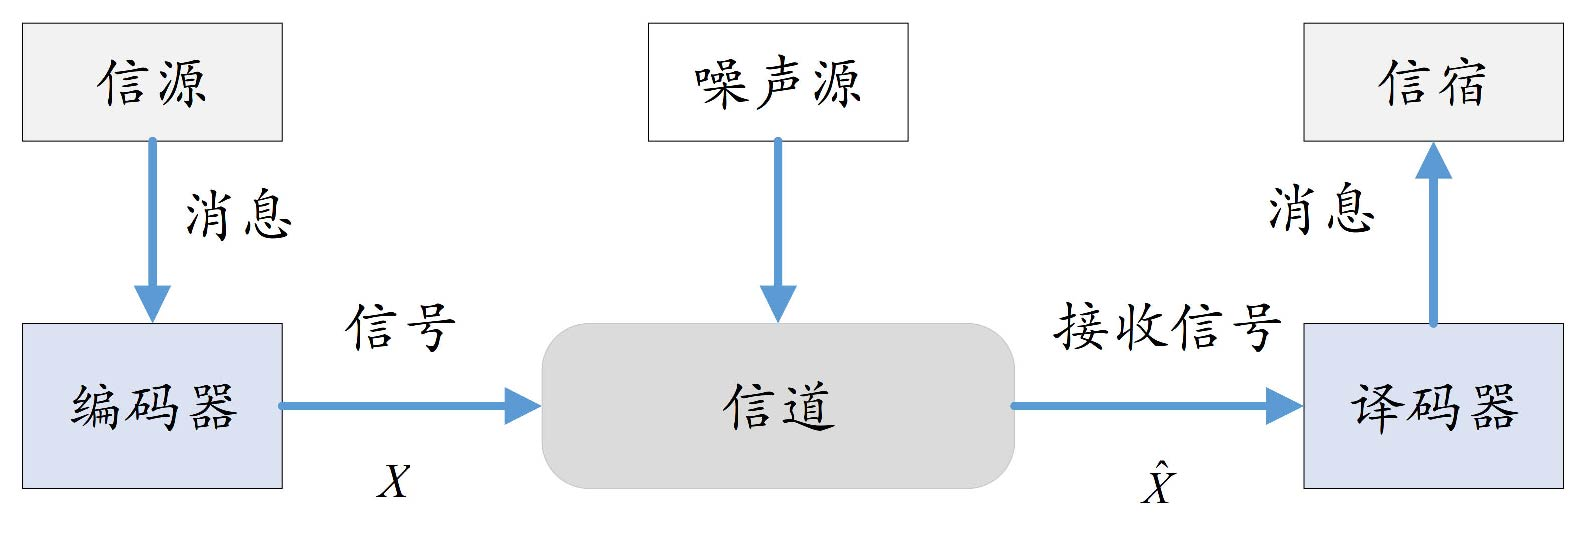
\includegraphics[width = 0.65\linewidth]{./figures/chapter03_1.jpg}
	\caption{Shannon基本通信系统模型}
	\label{fig:chapter03-communication-model}
\end{figure}

通信系统的信道数学模型$\left\{X~ Q(\hat{X}|X)~\hat{X}\right\}$刻画了随机变量$X\in\{x_1,x_2,\cdots,x_n\}$和$\hat{X}\in\{\hat{x}_1,\hat{x}_2,\cdots,\hat{x}_m\}$之间的依赖性。围绕通信系统中存在的问题,Shannon信息论的核心包括基本的熵定义和三大编码定理,具体是信息熵$H(X)$、条件熵$H(\hat{X}|X)$、联合熵$H(X,\hat{X})$、互信息量$I(X;\hat{X})$等定义,无失真信源编码定理、信道编码定理和限失真编码定理\cite{shannon1948a,Shannon1959Coding,cover2006elements}。信息论解决了通信过程中信息度量、临界数据压缩、临界通信传输速率的问题。以下简单介绍与本文密切相关的,基本且关键的定义及结论。
\subsection{信息熵}
为解决信息度量的问题,Shannon提出信息熵的概念,用于定量化描述随机变量$X$的不确定度。信息熵$H(X)$实际上是关于随机变量$X$分布的泛函数,独立于$X$的具体取值$x$,而仅依赖于支撑集上的概率分布函数$p(x)$\cite{cover2006elements}。
\begin{definition}\label{def:entropy}一个离散型随机变量$X$,取值于字母表空间$\mathcal{X}$,概率分布函数$p(x)={\rm Pr}\left\{X=x\right\}$,$x \in \mathcal{X}$,则随机变量$X$的信息熵$H(X)$定义为
\begin{equation}
H(X)=-\sum_{x\in \mathcal{X}}p(x)\log p(x)
\end{equation}
\end{definition}
上述定义\ref{def:entropy}定义了单个离散型随机变量的信息熵,描述了随机变量$X$具有的不确定度。该定义可以被推广到二元以及多元随机变量的情景定义联合信息熵。对于二元联合随机变量$(X,\hat{X})$,给出以下联合信息熵的定义
\begin{definition}
	二元离散型随机变量$(X,\hat{X})$,取值于字母表空间$\mathcal{X}\times \hat{\mathcal{X}}$,联合概率分布为$p(x,\hat{x})$,$x \in \mathcal{X},\hat{x} \in \hat{\mathcal{X}}$,由此,联合信息熵$H(X,\hat{X})$定义为
		\begin{alignat}{2}
		H(X,\hat{X})
		& 	=-\sum_{x\in \mathcal{X}}\sum_{\hat{x}\in \hat{\mathcal{X}}}p(x,\hat{x})\log p(x,\hat{x})\\
		& 	= -\sum_{x\in \mathcal{X}}\sum_{\hat{x}\in \hat{\mathcal{X}}}p(x,\hat{x}) \log p(x) q(\hat{x}|x)\\
		& = - \sum_{x \in \mathcal{X}}p(x) \log p(x)- \sum_{x\in \mathcal{X}}\sum_{\hat{x}\in \hat{\mathcal{X}}}p(x,\hat{x}) \log  q(\hat{x}|x)\\
		&   = H(X)+H(\hat{X}|X)\label{eq:chapter02-2.6}
	\end{alignat}
\end{definition}
上式~\ref{eq:chapter02-2.6}~中$H(\hat{X}|X)$是利用条件概率$q(\hat{x}|x)$定义的条件熵,表示随机变量$\hat{X}$在给定随机变量$X$时的不确定度,刻画了随机变量$\hat{X}$对变量$X$的影响。事实上,条件熵$H(\hat{X}|X)$是关于随机变量$X$的期望值。
\begin{definition}\label{def:condition_entropy}
		二元离散型随机变量$(X,\hat{X})$,取值于字母表空间$\mathcal{X}\times \hat{\mathcal{X}}$,联合概率分布为$p(x,\hat{x})$,$x \in \mathcal{X},\hat{x} \in \hat{\mathcal{X}}$,条件熵$H(\hat{X}|X)$表示为
 \begin{alignat}{2}
   H(\hat{X}|X)
   & = -\sum_{x \in \mathcal{X}}\sum_{\hat{x}\in \hat{\mathcal{X}}}p(x,\hat{x})\log q(\hat{x}|x)\\
   & = -\mathbb{E} \log p(\hat{X}|X)
   \end{alignat}

\end{definition}
基于上述定义\ref{def:condition_entropy},联合信息熵由二元离散型随机变量推广到多元随机变量时,则有多元随机变量的熵等于条件熵的加和,也就是熵的链式法则。%,具体的表述是

\begin{theorem}\label{theorm:multi_joint_entropy_}
	多元随机变量$X_1,X_2,\cdots,X_n$服从联合概率分布$p(x_1,x_2,\cdots,x_n)$,则联合信息熵
	\begin{equation}\label{eq:joint_entropy}
	H(X_1,X_2,\cdots,X_n)=\sum_{i=1}^{n}H(X_i|X_{i-1},\cdots,X_1)
	\end{equation}
\end{theorem}
\subsection{相对熵与互信息}\label{sec:entropty_mutual_information}
相对熵(Relative Entropy),也称为Kullback-Leibler\cite{cover2006elements,erven2014renyi}距离,主要用于度量两个概率分布之间的``距离''。相对熵总是非负的,非对称的,不满足三角不等式。
\begin{definition}
	假设$p(x)$,$q(x)$为支撑集$\mathcal{X}$上的两个概率分布函数,则它们之间的相对熵或Kullback-Leibler距离$D_{KL}(\cdot||\cdot)$定义为
	\begin{alignat}{2}
		D_{KL}(p||q)
		& =\sum_{x \in \mathcal{X}}p(x) \log \frac{p(x)}{q(x)}\\
		& 	 = \mathbb{E}_{p}\log \frac{p(x)}{q(x)}
	\end{alignat}
\end{definition}
互信息(Mutual Information,MI)是Shannon信息论中一个重要的概念,它是一个随机变量$\hat{X}$包含另一个随机变量$X$信息量的度量,量化有关$X$不确定度的减少量。基于通信系统观察者角度的不同,互信息可以有三种不同的语义解释,表达了不同的含义。此外,互信息与相对熵具有密切的关系,基于此,借鉴相对熵的表述,互信息可以定义为如下表述形式。
\begin{definition}
	假设$X,\hat{X}$为两个随机变量,$p(x,\hat{x})$为两随机变量的联合概率分布,$p(x)$和$p(\hat{x})$分别为对应的边缘概率分布。则随机变量$X$ 和$\hat{X}$之间的互信息为
	%\begin{equation}
%		I(X;\hat{X})=\sum_{x\in \mathcal{X}}\sum_{\hat{x}\in \hat{\mathcal{X}}}p(x,\hat{x})\log \frac{p(x,\hat{x})}{p(x)p(\hat{x})}
%	\end{equation}
	\begin{alignat}{2}
		I(X;\hat{X})
		& = D_{KL}\left(p(x,\hat{x})||p(x)p(\hat{x})\right)\\
		& = \sum_{x\in \mathcal{X}}\sum_{\hat{x}\in \hat{\mathcal{X}}}p(x,\hat{x})\log \frac{p(x,\hat{x})}{p(x)p(\hat{x})}
	\end{alignat}
\end{definition}
从通信的角度分析,互信息$I(X;\hat{X})$量化接收者在观测到$\hat{X}$后有关原始消息$X$的不确定度减少量。由此,互信息可以表示为先验概率分布$p(x)$、 信道条件概率分布$q(\hat{x}|x)$的二元函数形式,即
\begin{alignat}{2}
		I(X;\hat{X}) & = \sum_{x\in\mathcal{X}}\sum_{\hat{x}\in \hat{\mathcal{X}}}p(x)q(\hat{x}|x)\log \frac{p(x|\hat{x})}{p(x)}\\
		& =  -\sum_{x\in\mathcal{X}}\sum_{\hat{x}\in \hat{\mathcal{X}}}p(x)q(\hat{x}|x) \log p(x)-\left( -\sum_{x\in\mathcal{X}}\sum_{\hat{x}\in \hat{\mathcal{X}}} p(x)q(\hat{x}|x) \log p(x|\hat{x})\right)\\
		& = -\sum_{x \in \mathcal{X}}p(x)\log p(x)-\left( -\sum_{x\in\mathcal{X}}\sum_{\hat{x}\in \hat{\mathcal{X}}}p(x,\hat{x})\log p(x|\hat{x})\right)\\
		& =H(X)-H(X|\hat{X})
\end{alignat}

对称地,容易得到$I(X;\hat{X})=H(\hat{X})-H(\hat{X}|X)$。
\subsection{数据处理不等式}
\begin{definition}\label{def:dataprocessinginequality}
	离散型随机变量$X,\hat{X},Z$构成马尔可夫(Markov)链$X \rightarrow \hat{X}\rightarrow Z$的关系,则有互信息满足$I(X;\hat{X})\geq I(X;Z)$。
\end{definition}
数据处理不等式(Data Processing Inequality)表明信息的后处理过程降低了有效的信息量,增加了信息损失。在隐私保护研究中,数据处理不等式可以用于量化互信息的隐私泄露的边界。
\subsection{费诺不等式}
对任意的离散型随机变量$X$和$\hat{X}$,误差概率$P_e={\rm Pr}\left\{X \neq \hat{X}\right\}$,费诺不等式(Fano's Inequality)建立了随机变量$X$ 的与它的条件熵$H(X|\hat{X})$之间的关系,即
\begin{equation}
	H(P_e)+P_e\log |\mathcal{X}| \geq H(X|\hat{X})
\end{equation}
此外,结合互信息结论$I(X;\hat{X})=H(X)-H(X|\hat{X})$,容易得到下述推论~\ref{cor:chapter02-1}叙述的一个较强条件的费诺不等式结果。
\begin{corollary}\label{cor:chapter02-1}任意的离散型随机变量$X$和$\hat{X}$,取值于离散集合$\mathcal{X}$,设$P_e={\rm Pr}\left\{X \neq \hat{X}\right\}$为误差概率,则有
	\begin{equation}
	I(X;\hat{X})\geq H(X)-H(P_e)-P_e\log (|\mathcal{X}|-1)
	\end{equation}
\end{corollary}


\subsection{率失真理论}
1959年,Shannon发表题为《Coding Theorems for A Discrete Source With A Fidelity Criterion》\cite{Shannon1959Coding}的文章,提出了满足保真度准则的限失真编码定理,也就是著名的率失真理论。率失真理论解决了临界通信传输率的问题,也就是,对于给定的信源概率分布$p(x)$与失真度量函数$d(x,\hat{x})$,在满足限失真门限$\delta$条件下,数据损失压缩达到的最小信息传输率$R(\delta)$。
\begin{definition}
失真度量函数$d(x,\hat{x}),x\in \mathcal{X},\hat{x}\in \hat{\mathcal{X}}$是信源字母表$\mathcal{X}$与再生字母表$ \hat{\mathcal{X}}$乘积空间到非负实数的函数映射$d:\mathcal{X}\times \hat{\mathcal{X}}\rightarrow \mathbb{R}^{+}$。
\end{definition}
失真函数$d(x,\hat{x})$测量符号$\hat{x}$表示$x$时的失真距离,期望失真$\mathbb{E}[d(x,\hat{x})]$定量的描述噪声信道的统计特性。在率失真区域$(R,\delta)$中所有码率$R$的下确界称为率失真函数,由此,则有下述的定义。
\begin{definition}
	对于给定的失真门限$\delta$和失真度量函数$d(x,\hat{x})$,在满足$(R,\delta)$的失真区域,所有码率$R$的下确界称为率失真函数$R(\delta)$
	\begin{alignat}{2}
	R(\delta) & = \min_{q(\hat{x}|x)}I(X;\hat{X}) \nonumber \\
	  \mbox{\textup{subject to}}\quad 
      & \sum_{x}\sum_{\hat{x}}p(x)q(\hat{x}|x)d(x,\hat{x})\leq \delta\\
	  &  \sum_{\hat{x} \in \mathcal{X}}q(\hat{x}|x)=1, \forall x \in \mathcal{X}\\
	  &  q(\hat{x}|x) \geq 0, \forall x \in \mathcal{X}, \hat{x} \in \hat{\mathcal{X}}
	\end{alignat}
%	\begin{equation}
%	R(\delta) = \min_{q(\hat{x}|x):\sum_{x}\sum_{\hat{x}}p(x)q(\hat{x}|x)d(x,\hat{x})\leq \delta}I(X;\hat{X})
%	\end{equation}
其中,$p(x)$为信源概率分布,$q(\hat{x}|x)$为信道条件概率分布。
\end{definition}

\section{优化与均衡理论}
优化与均衡是利用最优性选择解决约束问题的工具,属于重要的数学优化问题研究范畴。近年来,在差分隐私的研究中,定义于凸集中的凸函数最优性可用于设计最优化隐私保护的机制,解决隐私与效用的权衡问题。借鉴均衡的最优性思想,可用于解决隐私保护策略最优性选择问题。为了更好的阐述本文后续的研究工作,本节中给出本文研究所使用的凸优化及均衡理论基础。
\subsection{优化问题}
通常情况下,优化问题由目标函数和约束条件表达式两部分组成,一个标准形式的优化问题\cite{boyd2004convex}具有如下形式
 \begin{alignat}{2}
   \mbox{minimize}\quad & f_{0}(x) \nonumber\\
   \mbox{subject to} \quad
   & f_i(x)\leq 0,\quad i \in\{1,2,\cdots,m\} \\
   & h_j(x)=0,\quad j\in \left\{1,2,\cdots,p\right\}
   \end{alignat}
其中的$x\in \mathbb{R}^{n}$,上述优化问题的最优解$p^{*}$满足
$p^{*}=\inf \left\{f_0(x)|f_i(x)\leq 0, h_j(x)=0\right\}$,$i \in\left\{1,2,\cdots,m\right\},j\in\left\{1,2,\cdots,p\right\}$。对上述最优化问题构造拉格朗日对偶函数
\begin{equation}
	L(x,\lambda,\mu)=f_0(x)+\sum_{i=1}^{m}\lambda_i f_i(x)+\sum_{j=1}^{p}\mu_j h_j(x)
\end{equation}
进行求解,其中的$\lambda_i$是第$i$个不等式约束$f_i(x)\leq 0$条件的拉格朗日乘子。与上式对应的,$\mu_j$是第$j$个等式约束条件$h_j(x)=0$的拉格朗日乘子。通过求解最优性条件可以得到目标函数$f_{0}(x)$的最小值。

凸优化问题是一类特殊而重要的优化问题,它要求目标函数和不等式约束函数必须是凸的,等式约束函数$a_i^T x = b_i$必须是仿射的\cite{boyd2004convex}。 由于篇幅的限制,在此省略对于凸集、凸函数、凸组合的介绍。

\subsection{对策博弈}
隐私保护系统中隐私与数据可用性是一对相互依存的矛盾冲突问题,根据隐私与效用原则\cite{sankar2013utility},该问题属于极大极小的对偶问题。针对该问题,寻找一种权衡折中的隐私保护技术方案实现隐私与效用的均衡是一种较为理想的选择。鉴于此,借鉴对策博弈的思想构造隐私保护的对策博弈,成为一种行之有效的分析方法。标准形式的对策博弈模型具有如下的形式。
\begin{definition}对策博弈定义为$G=(N,S,U)$,其中,$N=\{1,2,\cdots,n\}$表示参与者集合,$S=\{S_1,S_2,\cdots,S_n\}$分别表示参与者的策略空间,$U:S_1 \times S_2 \times \cdots \times S_n \rightarrow \mathbb{R}$是参与者效用函数。对于任意的$i\in N$,$s_i$和$s_{-i}$分别表示第$i$ 个参与者和其它$i-1$个参与者策略组合,$U_i(s_i,s_{-i})$表示第$i$个参与者的效用(收益)。
\end{definition}

对于有限策略的对策博弈,$N$和$S$分别为有限集合,效用度量是冯$\cdot$诺依曼-摩根斯坦效用函数(von Neumann-Morgenstern Utility Function)。 博弈中的参与者被假设为理性玩家,偏好于收益最大化的策略。由此,博弈的Nash均衡定义为
\begin{definition}[Nash均衡]对策博弈$G=(N,S,U)$中,对任意的参与者$i (i\in N)$,存在$s_i^* \in S_i$使得效用函数满足
	\begin{equation}
		U_i(s_i^*,s_{-i}) \geq U_i(s_i,s_{-i})
	\end{equation}
对所有的$s_i \in S_{i}$,则策略组合$(s_1,s_2,\cdots,s_n)$是博弈$G$的Nash均衡。
\end{definition}

通常情况下,隐私保护系统仅涉及到隐私保护者与隐私分析者或称为敌手,它可以看作仅有两方参与者\cite{dwork2014algorithmic}。基于隐私保护的目标,从隐私泄露的角度分析,隐私保护系统是有关隐私保护者和敌手的攻防博弈,属于二人博弈。
\begin{definition}
在二人矩阵博弈$(A,B)$,其中$A$和$B$是$m\times n$矩阵,分别表示参与者$1$和$2$的收益,矩阵的$m$行和$n$列分别对应于参与者$1$和$2$的可行策略。若收益矩阵满足$B=-A$,则该博弈是二人零和博弈(Two-Person Zero-Sum,TPZS)。
\end{definition}

二人零和博弈模型中,参与者$1$选择策略旨在最大化其收益,对应的参与者$2$偏好于最小化损失的策略。由此,二人零和博弈中存在对立冲突竞争参与者的目标,鞍点是它稳定的均衡点。鞍点的存在性由极大极小的定理保障,以下给出简要的叙述。
\begin{theorem}[von Neumann's Minimax Theorem \cite{du1995minimax}]\label{theorem:minmax}假设$S_1$和$S_2$为两个非空的、紧致的欧几里德空间凸子集,函数$U(s_1,s_2)$是一个连续函数,满足$U(s_1,s_2)$是关于$s_1 \in S_1$的凸函数对所有的$s_2 \in S_2$,同时,$U(s_1,s_2)$是$s_2 \in S_2$的凹函数对所有的$s_1 \in S_1$,则有下式成立
\begin{equation}
	\sup_{s_2\in S_2}\inf_{ s_1\in S_1} U(s_1,s_2)= \inf_{ s_1\in S_1}\sup_{s_2\in S_2}U(s_1,s_2)
\end{equation}
\end{theorem}

基于上述定理\ref{theorem:minmax},若$(s_1^*,s_2^*)$是函数$U(s_1,s_2)$的一个鞍点,则它是对策博弈的一个解,满足$U(s_1,s_2^*)\leq U(s_1^*,s_2^*)\leq U(s_1^*,s_2)$。
\subsection{凹凸博弈}\label{sec:chapter3_convex_concave_game}
冯$\cdot$诺依曼(von Neumann)极大极小定理利用了函数的凹凸性质,该性质在著名的凹凸博弈模型有重要的作用。凹凸博弈中收益函数有其特殊的结构形式,它是一个参与者策略的凸函数,另一个参与者策略的凹函数。这种形式的对策博弈的均衡是每个参与者的纯策略组合。鉴于此,则有以下参与者最佳响应策略。
\begin{theorem}\label{theorem:extence_saddlepoint}
	假设$S_1$和$S_2$是封闭有界的欧几里德空间非空凸子集,收益函数$U(s_1,s_2)$是关于$s_1 \in S_1$和$s_2 \in S_2$的连续函数。若$U(s_1,s_2)$ 是一个关于$s_1$的凹函数,则参与者$1$的最佳纯策略响应$s_1^* $使得$v= \max_{s_1} \min_{s_2}U(s_1,s_2)$。同样地,$U(s_1,s_2)$是一个关于$s_2$ 的凸函数,则参与者$2$的最佳纯策略响应$s_2^* $使得$ v=  \min_{s_2}\max_{s_1}U(s_1,s_2)$。
\end{theorem}
定理\ref{theorem:extence_saddlepoint}是二人零和博弈鞍点的存在性定理,它表达出了凹凸博弈鞍点的计算是寻找策略组合$(s_1^*,s_2^*)$使得它是参与者$1$和$2$的最佳响应策略。
\section{差分隐私的均衡优化}
本章中,定义\ref{def:chapter03-privacy_leakage}首先给出了隐私泄露的界定,随后,介绍了隐私保护的本质,其主要目标是在维持数据可用性的条件下保护用户个体的隐私。基于数据失真扰动的差分隐私模型是目前学术研究的主要焦点,其重点在于设计差分隐私机制解决隐私与数据可用性的矛盾问题。{\em 事实上,差分隐私中难以实现完美的隐私保护,达到完全的无隐私泄露,由此,关注的问题只能寻找一种权衡折中的解决方案。}鉴于此分析,本文旨在利用信息论、优化理论以及均衡理论研究差分隐私的均衡优化模型及算法获得最优性隐私机制,这成为一种较为理想的解决方案。以下给出本文中均衡优化的研究范畴界定。

\begin{definition}\label{def:chapter03_equilibrium_optimation}
	针对不同差分隐私应用中隐私与数据效用需求,差分隐私的均衡优化是研究约束数据质量损失条件下,设计最小化隐私泄露风险的隐私机制。其次,在可达的隐私机制集合中,寻找最优的差分隐私保护策略。目标是优化隐私保护机制,获得隐私与数据可用性的均衡。
\end{definition}

基于上述定义\ref{def:chapter03_equilibrium_optimation},为了在差分隐私框架下获得隐私保护与数据效用(数据可用性)的均衡,需要解决几个关键的问题。{\em 首先,隐私泄露与数据效用的度量问题,它们是研究差分隐私机制设计的基础。其次,针对应用场景中的隐私保护需求,建立差分隐私的均衡优化模型是一个关键问题。最后,针对提出的均衡优化模型,设计有效的算法也是个关键的问题。}围绕这些问题的解决,开展了本文的研究工作,后续章节分别介绍本文对于差分隐私均衡优化模型与算法的具体研究工作。
\section{本章小结}

围绕本文的研究工作,本章首先介绍了隐私以及隐私泄露的定义,明确了本文中隐私保护的研究范畴,随后,介绍了差分隐私模型并给出标准形式的定义。其次,介绍了本文研究需要的Shannon信息论知识,包括基本通信模型、信息熵、条件熵、联合熵、互信息量等概念。在此基础上,对信息论中两个重要的不等式和率失真理论进行了简要的叙述。进一步,介绍了本文将使用的优化理论知识以及在对策博弈模型中的应用。最后,结合本章内容,给定了本文中所研究的差分隐私均衡优化的定义。针对差分隐私模型中隐私保护与数据可用性之间的矛盾问题,利用均衡优化思想研究差分隐私最优化机制是本文研究的核心。本章中所介绍内容为后续章节提供了基本模型与定义,是开展后续研究工作的理论出发点。
